\documentclass[]{article}
\usepackage[left=1in,top=1in,right=1in,bottom=1in]{geometry}


%%%% more monte %%%%
% thispagestyle{empty}
% https://stackoverflow.com/questions/2166557/how-to-hide-the-page-number-in-latex-on-first-page-of-a-chapter
\usepackage{color}
% \usepackage[table]{xcolor} % are they using color?

% \definecolor{WSU.crimson}{HTML}{981e32}
% \definecolor{WSU.gray}{HTML}{5e6a71}

% \definecolor{shadecolor}{RGB}{248,248,248}
\definecolor{WSU.crimson}{RGB}{152,30,50} % use http://colors.mshaffer.com to convert from 981e32
\definecolor{WSU.gray}{RGB}{94,106,113}

%%%%%%%%%%%%%%%%%%%%%%%%%%%%

\newcommand*{\authorfont}{\fontfamily{phv}\selectfont}
\usepackage{lmodern}


  \usepackage[T1]{fontenc}
  \usepackage[utf8]{inputenc}




\usepackage{abstract}
\renewcommand{\abstractname}{}    % clear the title
\renewcommand{\absnamepos}{empty} % originally center

\renewenvironment{abstract}
 {{%
    \setlength{\leftmargin}{0mm}
    \setlength{\rightmargin}{\leftmargin}%
  }%
  \relax}
 {\endlist}

\makeatletter
\def\@maketitle{%
  \pagestyle{empty}
  \newpage
%  \null
%  \vskip 2em%
%  \begin{center}%
  \let \footnote \thanks
    {\fontsize{18}{20}\selectfont\raggedright  \setlength{\parindent}{0pt} \@title \par}%
}
%\fi
\makeatother






\usepackage{color}
\usepackage{fancyvrb}
\newcommand{\VerbBar}{|}
\newcommand{\VERB}{\Verb[commandchars=\\\{\}]}
\DefineVerbatimEnvironment{Highlighting}{Verbatim}{commandchars=\\\{\}}
% Add ',fontsize=\small' for more characters per line
\usepackage{framed}
\definecolor{shadecolor}{RGB}{248,248,248}
\newenvironment{Shaded}{\begin{snugshade}}{\end{snugshade}}
\newcommand{\AlertTok}[1]{\textcolor[rgb]{0.94,0.16,0.16}{#1}}
\newcommand{\AnnotationTok}[1]{\textcolor[rgb]{0.56,0.35,0.01}{\textbf{\textit{#1}}}}
\newcommand{\AttributeTok}[1]{\textcolor[rgb]{0.77,0.63,0.00}{#1}}
\newcommand{\BaseNTok}[1]{\textcolor[rgb]{0.00,0.00,0.81}{#1}}
\newcommand{\BuiltInTok}[1]{#1}
\newcommand{\CharTok}[1]{\textcolor[rgb]{0.31,0.60,0.02}{#1}}
\newcommand{\CommentTok}[1]{\textcolor[rgb]{0.56,0.35,0.01}{\textit{#1}}}
\newcommand{\CommentVarTok}[1]{\textcolor[rgb]{0.56,0.35,0.01}{\textbf{\textit{#1}}}}
\newcommand{\ConstantTok}[1]{\textcolor[rgb]{0.00,0.00,0.00}{#1}}
\newcommand{\ControlFlowTok}[1]{\textcolor[rgb]{0.13,0.29,0.53}{\textbf{#1}}}
\newcommand{\DataTypeTok}[1]{\textcolor[rgb]{0.13,0.29,0.53}{#1}}
\newcommand{\DecValTok}[1]{\textcolor[rgb]{0.00,0.00,0.81}{#1}}
\newcommand{\DocumentationTok}[1]{\textcolor[rgb]{0.56,0.35,0.01}{\textbf{\textit{#1}}}}
\newcommand{\ErrorTok}[1]{\textcolor[rgb]{0.64,0.00,0.00}{\textbf{#1}}}
\newcommand{\ExtensionTok}[1]{#1}
\newcommand{\FloatTok}[1]{\textcolor[rgb]{0.00,0.00,0.81}{#1}}
\newcommand{\FunctionTok}[1]{\textcolor[rgb]{0.00,0.00,0.00}{#1}}
\newcommand{\ImportTok}[1]{#1}
\newcommand{\InformationTok}[1]{\textcolor[rgb]{0.56,0.35,0.01}{\textbf{\textit{#1}}}}
\newcommand{\KeywordTok}[1]{\textcolor[rgb]{0.13,0.29,0.53}{\textbf{#1}}}
\newcommand{\NormalTok}[1]{#1}
\newcommand{\OperatorTok}[1]{\textcolor[rgb]{0.81,0.36,0.00}{\textbf{#1}}}
\newcommand{\OtherTok}[1]{\textcolor[rgb]{0.56,0.35,0.01}{#1}}
\newcommand{\PreprocessorTok}[1]{\textcolor[rgb]{0.56,0.35,0.01}{\textit{#1}}}
\newcommand{\RegionMarkerTok}[1]{#1}
\newcommand{\SpecialCharTok}[1]{\textcolor[rgb]{0.00,0.00,0.00}{#1}}
\newcommand{\SpecialStringTok}[1]{\textcolor[rgb]{0.31,0.60,0.02}{#1}}
\newcommand{\StringTok}[1]{\textcolor[rgb]{0.31,0.60,0.02}{#1}}
\newcommand{\VariableTok}[1]{\textcolor[rgb]{0.00,0.00,0.00}{#1}}
\newcommand{\VerbatimStringTok}[1]{\textcolor[rgb]{0.31,0.60,0.02}{#1}}
\newcommand{\WarningTok}[1]{\textcolor[rgb]{0.56,0.35,0.01}{\textbf{\textit{#1}}}}



\title{\textbf{\textcolor{WSU.crimson}{The Difference Between You and An
NBA Player.}} \newline \textbf{\textcolor{WSU.gray}{Comparing the Ape
Indexes of NBA Players and Ordinary Males.}}  }
 

%  

% \author{ \Large true \hfill \normalsize \emph{} }
\author{\Large Nahom
Debela\vspace{0.05in} \newline\normalsize\emph{Washington State
University}  }


\date{November 11, 2020}
\setcounter{secnumdepth}{3}

\usepackage{titlesec}
% See the link above: KOMA classes are not compatible with titlesec any more. Sorry.
% https://github.com/jbezos/titlesec/issues/11
\titleformat*{\section}{\bfseries}
\titleformat*{\subsection}{\bfseries\itshape}
\titleformat*{\subsubsection}{\itshape}
\titleformat*{\paragraph}{\itshape}
\titleformat*{\subparagraph}{\itshape}

% https://code.usgs.gov/usgs/norock/irvine_k/ip-092225/


%\titleformat*{\section}{\normalsize\bfseries}
%\titleformat*{\subsection}{\normalsize\itshape}
%\titleformat*{\subsubsection}{\normalsize\itshape}
%\titleformat*{\paragraph}{\normalsize\itshape}
%\titleformat*{\subparagraph}{\normalsize\itshape}

% https://tex.stackexchange.com/questions/233866/one-column-multicol-environment#233904
\usepackage{environ}
\NewEnviron{auxmulticols}[1]{%
  \ifnum#1<2\relax% Fewer than 2 columns
    %\vspace{-\baselineskip}% Possible vertical correction
    \BODY
  \else% More than 1 column
    \begin{multicols}{#1}
      \BODY
    \end{multicols}%
  \fi
}





\usepackage{natbib}
\setcitestyle{aysep={}} %% no year, comma just year
% \usepackage[numbers]{natbib}
\bibliographystyle{./../biblio/ormsv080.bst}



\usepackage[strings]{underscore} % protect underscores in most circumstances




\newtheorem{hypothesis}{Hypothesis}
\usepackage{setspace}


%%%%%%%%%%%%%%%%%%%%%%%%%%%%%%%%%%%%%%%%%%%%%%%%%%%%%
%%% MONTE ADDS %%%

\usepackage{fancyhdr} % fancy header 
\usepackage{lastpage} % last page 

\usepackage{multicol}


\usepackage{etoolbox}
\AtBeginEnvironment{quote}{\singlespacing\small}
% https://tex.stackexchange.com/questions/325695/how-to-style-blockquote


\usepackage{soul}			%% allows strike-through
\usepackage{url}			%% fixes underscores in urls
\usepackage{csquotes}		%% allows \textquote in references
\usepackage{rotating}		%% allows table and box rotation
\usepackage{caption}		%% customize caption information
\usepackage{booktabs}		%% enhance table/tabular environment
\usepackage{tabularx}		%% width attributes updates tabular
\usepackage{enumerate}		%% special item environment
\usepackage{enumitem}		%% special item environment

\usepackage{lineno}		%% allows linenumbers for editing using \linenumbers
\usepackage{hanging}


\usepackage{mathtools}  	%% also loads amsmath
\usepackage{bm}		%% bold-math
\usepackage{scalerel}	%% scale one element (make one beta bigger font)

\newcommand{\gFrac}[2]{ \genfrac{}{}{0pt}{1}{{#1}}{#2} }

\newcommand{\betaSH}[3]{  \gFrac{\text{\tiny #1}}{{\text{\tiny #2}}}\hat{\beta}_{\text{#3}}   }
\newcommand{\betaSB}[3]{              ^{\text{#1}} _{\text{#2}} \bm{\beta} _{\text{#3}}                   }  %% bold
\newcommand{\bigEQ}{  \scaleobj{1.5}{{\ }= } }
\newcommand{\bigP}[1]{  \scaleobj{1.5}{#1 } }





\usepackage{endnotes}  % he already does this ...
\renewcommand{\enotesize}{\normalsize}
% https://tex.stackexchange.com/questions/99984/endnotes-do-not-be-superscript-and-add-a-space
\renewcommand\makeenmark{\textsuperscript{[\theenmark]}} % in brackets %
% https://tex.stackexchange.com/questions/31574/how-to-control-the-indent-in-endnotes
\patchcmd{\enoteformat}{1.8em}{0pt}{}{}

\patchcmd{\theendnotes}
  {\makeatletter}
  {\makeatletter\renewcommand\makeenmark{\textbf{[\theenmark]} }}
  {}{}



% https://tex.stackexchange.com/questions/141906/configuring-footnote-position-and-spacing

\addtolength{\footnotesep}{5mm} % change to 1mm

\renewcommand{\thefootnote}{\textbf{\arabic{footnote}}}
\let\footnote=\endnote
%\renewcommand*{\theendnote}{\alph{endnote}}
%\renewcommand{\theendnote}{\textbf{\arabic{endnote}}}


\renewcommand*{\notesname}{ENDNOTES}

\makeatletter
\def\enoteheading{\section*{\notesname
  \@mkboth{\MakeUppercase{\notesname}}{\MakeUppercase{\notesname}}}%
  \mbox{}\par\vskip-2.3\baselineskip\noindent\rule{.5\textwidth}{0.4pt}\par\vskip\baselineskip}
\makeatother


\renewcommand*{\contentsname}{TABLE OF CONTENTS}

\renewcommand*{\refname}{REFERENCES}


%\usepackage{subfigure}
\usepackage{subcaption}

\captionsetup{labelfont=bf}  % Make Table / Figure bold

%%% you could add elements here ... monte says .... %%%
%\usepackage{mypackageForCapitalH}


%%%%%%%%%%%%%%%%%%%%%%%%%%%%%%%%%%%%%%%%%%%%%%%%%%%%%

% set default figure placement to htbp
\makeatletter
\def\fps@figure{htbp}
\makeatother


% move the hyperref stuff down here, after header-includes, to allow for - \usepackage{hyperref}

\makeatletter
\@ifpackageloaded{hyperref}{}{%
\ifxetex
  \PassOptionsToPackage{hyphens}{url}\usepackage[setpagesize=false, % page size defined by xetex
              unicode=false, % unicode breaks when used with xetex
              xetex]{hyperref}
\else
  \PassOptionsToPackage{hyphens}{url}\usepackage[draft,unicode=true]{hyperref}
\fi
}

\@ifpackageloaded{color}{
    \PassOptionsToPackage{usenames,dvipsnames}{color}
}{%
    \usepackage[usenames,dvipsnames]{color}
}
\makeatother
\hypersetup{breaklinks=true,
            bookmarks=true,
            pdfauthor={Nahom Debela (Washington State University)},
             pdfkeywords = {},  
            pdftitle={The Difference Between You and An NBA
Player.: Comparing the Ape Indexes of NBA Players and Ordinary Males.},
            colorlinks=true,
            citecolor=blue,
            urlcolor=blue,
            linkcolor=magenta,
            pdfborder={0 0 0}}
\urlstyle{same}  % don't use monospace font for urls

% Add an option for endnotes. -----

%
% add tightlist ----------
\providecommand{\tightlist}{%
\setlength{\itemsep}{0pt}\setlength{\parskip}{0pt}}

% add some other packages ----------

% \usepackage{multicol}
% This should regulate where figures float
% See: https://tex.stackexchange.com/questions/2275/keeping-tables-figures-close-to-where-they-are-mentioned
\usepackage[section]{placeins}



\pagestyle{fancy}   
\lhead{\textcolor{WSU.crimson}{\textbf{ The Difference Between You and
An NBA Player. }}}
\chead{}
\rhead{\textcolor{WSU.gray}{\textbf{  Page\ \thepage\ of\ \protect\pageref{LastPage} }}}
\lfoot{}
\cfoot{}
\rfoot{}


\begin{document}
	
% \pagenumbering{arabic}% resets `page` counter to 1 
%    

% \maketitle

{% \usefont{T1}{pnc}{m}{n}
\setlength{\parindent}{0pt}
\thispagestyle{plain}
{\fontsize{18}{20}\selectfont\raggedright 
\maketitle  % title \par  

}

{
   \vskip 13.5pt\relax \normalsize\fontsize{11}{12} 
   
\textbf{\authorfont Nahom Debela} \hskip 15pt \emph{\small Washington
State University}   

}

}








\begin{abstract}

    \hbox{\vrule height .2pt width 39.14pc}

    \vskip 8.5pt % \small 

\noindent \noindent In this report I walk through my steps in answering
my research questions. I seek to find relationships between NBA
measurement data and measurements from ordinary people. I perform
statistical data analysis to uncover trends and solve my questions.
\vspace{0.12in}


    



    
    \hbox{\vrule height .2pt width 39.14pc}
    \vskip 5pt 
    \hfill \textbf{\textcolor{WSU.gray}{ November 11, 2020 } }
    \vskip 5pt 
    
\end{abstract}


\vskip -8.5pt



 % removetitleabstract

\noindent  

\section{Introduction}
\label{sec:intro}

\begin{figure}[!ht]
    \begin{subfigure}[h]{0.4\textwidth}
    \centering
    %  trim={<left> <lower> <right> <upper>}
    % https://shantoroy.com/latex/add-subfig-in-latex/
            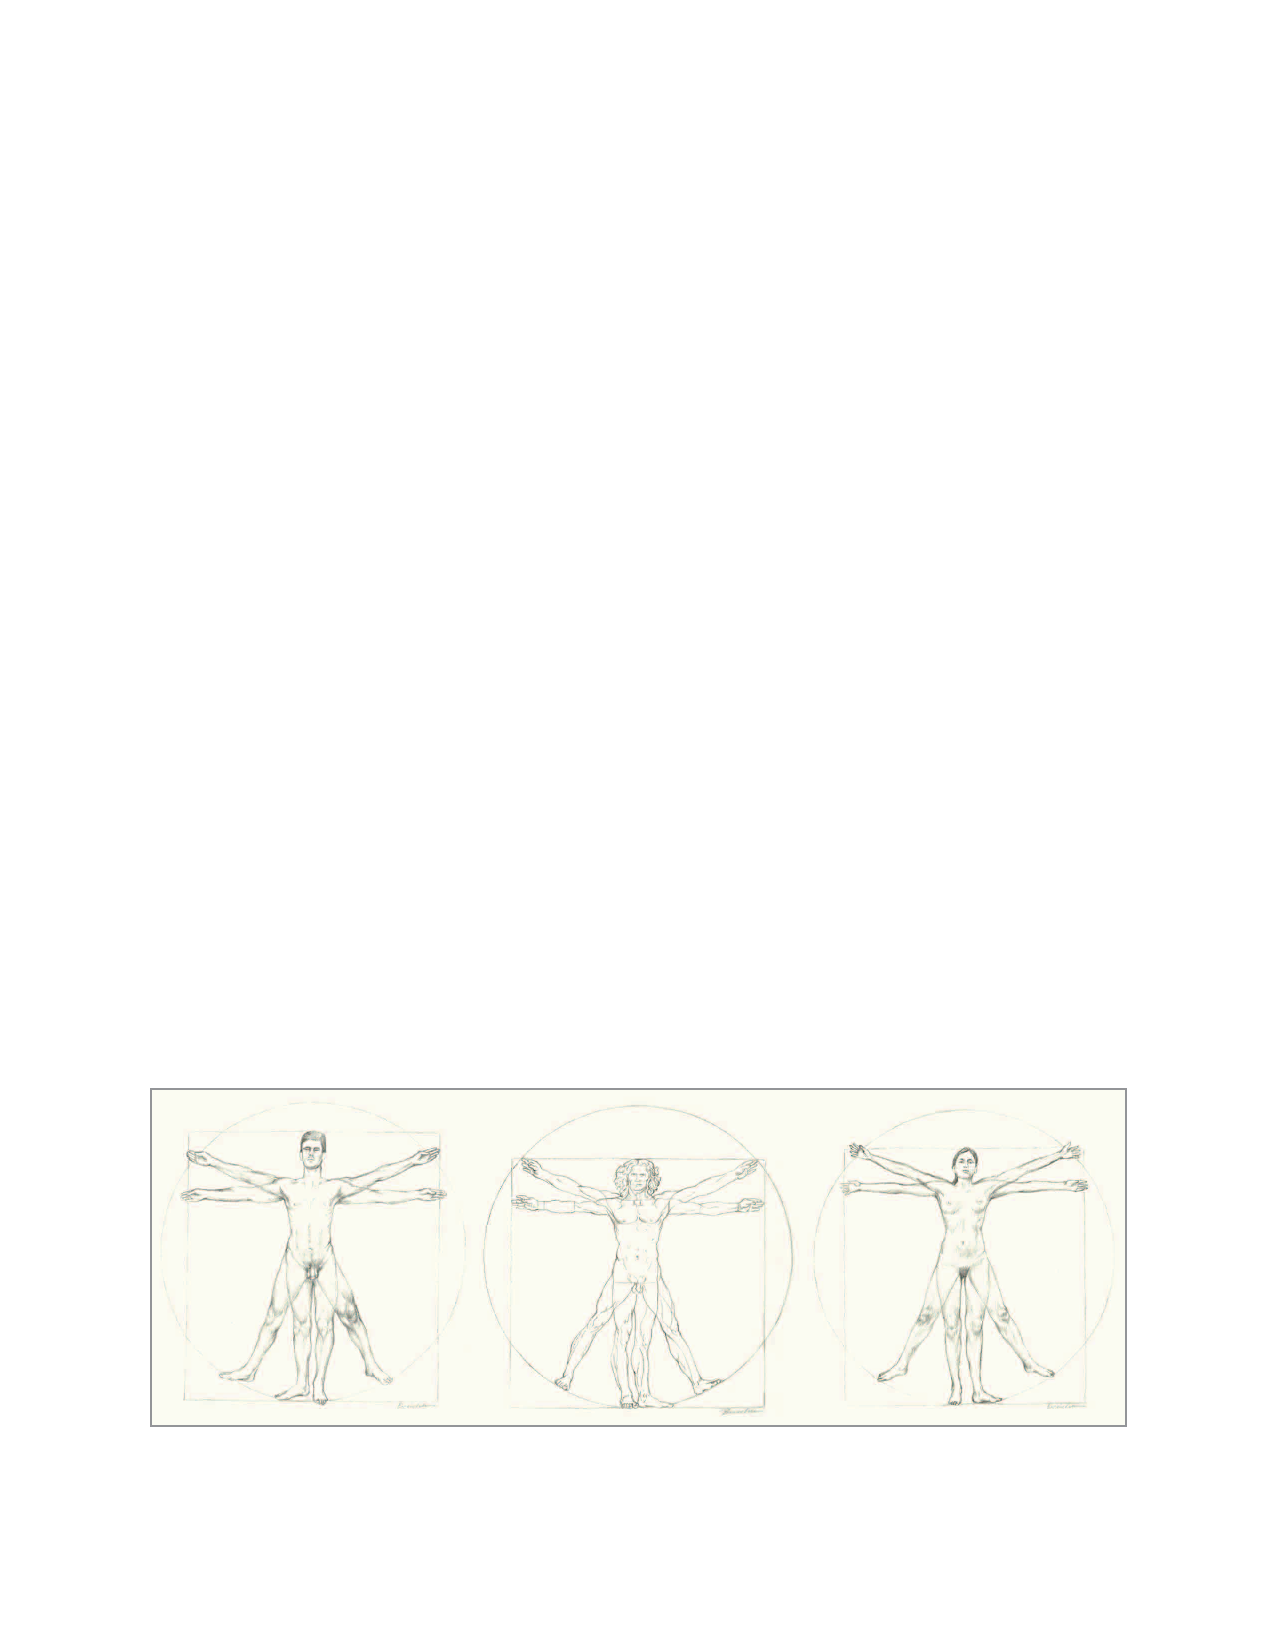
\includegraphics[trim = 0 0 11.25cm 0,clip,scale=1]{figures/Vitruvian.pdf}
        \caption{Figure 1: Male Vitruvian Figure }
        \label{fig:sub-first}
    \end{subfigure}
    \begin{subfigure}[h]{0.4\textwidth}
    \centering
        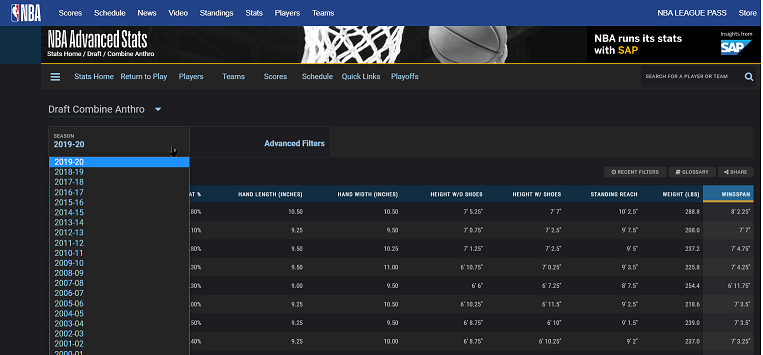
\includegraphics[trim =  0 0.5cm 4.0cm 0,clip,scale=1]{figures/nba.png}
            \caption{Figure 2: NBA Measurements}
        \label{fig:sub-second}
    \end{subfigure}
    \vspace{2.5mm}
    \hrule
    \vspace{2.5mm}
        \caption{\textbf{  }The Vitruvian drawing was made by Italian polymath Leonardo da Vinci in about 1490. It is based upon the theory that the human body can be symmetrically inscribed within both a circle and a square \newline  \newline   \textbf{Figure 2:} NBA Data of Measurements that were taken from the NBA website. }
        The
        \newline  \newline 
        \label{fig:combined}
    \vspace{-2.5mm}
    \hrule
\end{figure}

\newpage

\section{Research Question: How does the ratio between height and arm span compare between NBA players and normal males?}
\label{sec:rq}

\subsection{Is there a strong relationship between height and arm span?}
\label{sec:rq2}

\subsection{Has the ratio between height and arm span changed over time for NBA Players?}
\label{sec:rq3}

\begin{figure}[!ht]
    \hrule
    \caption{ \textbf{Wingpsan} }
    \begin{center}
        \scalebox{1.00}{    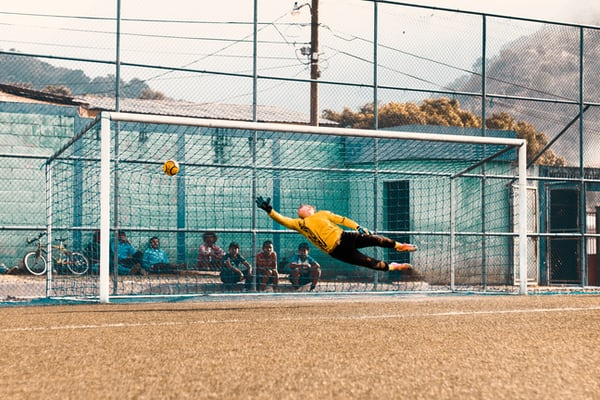
\includegraphics[trim = 0 0 0 0,clip,width=0.85\textwidth]{figures/reach.png} }
    \end{center}
    \label{fig:handout-1}
    \hrule
\end{figure}

\section{Data Description}
\label{sec:data}

I've used 3 separate data sets. One data set consists of measurement
data from participants who have filled out the handout. From this data I
have used ``Arm Span'',``Height'', and I have calculated ``Ape Index''.
Ape Index is simply the ratio between one's height and arm span. In my
analysis, I used Ape Index to observe if there is a relationship between
the average NBA players ape index and the ordinary person's ape index.
\newline \newline

\noindent The other 2 data sets are NBA measurent data from ``Kaggle''.
This dataset came as one file. I filtered the NBA data and split it into
2 separate data sets. One included previous NBA players that played in
2002 and before. The other contains recent NBA players who have played
in 2016 and after. For my analysis, I used: ``Arm Span'', ``Height'',
and I have calculated ``Ape Index'' for both time frames. These datasets
are helpful in answering: Does the ratio between height and arm span
change over time? \newpage

\subsection{Summary of Sample}
\label{sec:data-sample}

Gender: This is a factor. Possible values include, male, female, other.
100\% of my sample is ``male.''\vspace{2.5mm}

\noindent Units: All my observations are in cm.

\noindent Age: All my observations are samples where age is at least 18.

\noindent The rest of my data includes Height, Wingspan and Ape Scale
for all 3 datasets. \vspace{2.5mm} \label{sec:Summary of Sample}

\begin{figure}[!ht]
    \hrule
    \caption{ \textbf{Summary Table} }
    \begin{center}
        \scalebox{1.00}{    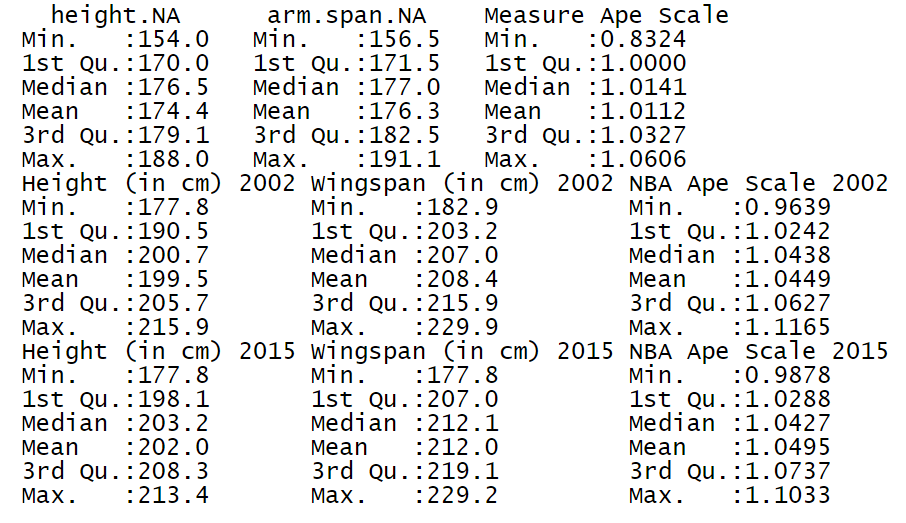
\includegraphics[trim = 0 0 0 0,clip,width=0.85\textwidth]{figures/summary.png} }
    \end{center}
    \label{fig:handout-1}
    \hrule
\end{figure}

\vspace{2.5mm}

\noindent From all 3 datasets the largest mean in Ape scale is in the
2015 NBA Data set.

\noindent Ape Scale seems to be the largest in the 2015 NBA dataset (M =
1.0495), followed by 2002 NBA Dataset (M=1.0449cm) and finally the
Normal measurement data (M=1.0112cm) \vspace{2.5mm}

\noindent Wingspan seems to be the largest in the 2015 NBA dataset (M =
212.0), followed by 2002 NBA Dataset (M=208.4cm) and finally the Normal
measurement data (M=176.3cm)

\noindent Wingpsan of NBA players in both datasets is on average larger
than the normal males wingspan by 33.9cm. \vspace{1mm}

\noindent Height seems to be the largest in the 2015 NBA dataset (M =
202.0), followed by 2002 NBA Dataset (M=199.5cm) and finally the Normal
measurement data (M=174.4cm)

\noindent Height of NBA players in both datasets is on average larger
than the normal males height by 26.4cm.

\newpage

\begin{figure}[!ht]
    \hrule
    \caption{ \textbf{Height vs Wingspan Plot} }
    \begin{center}
        \scalebox{1.00}{    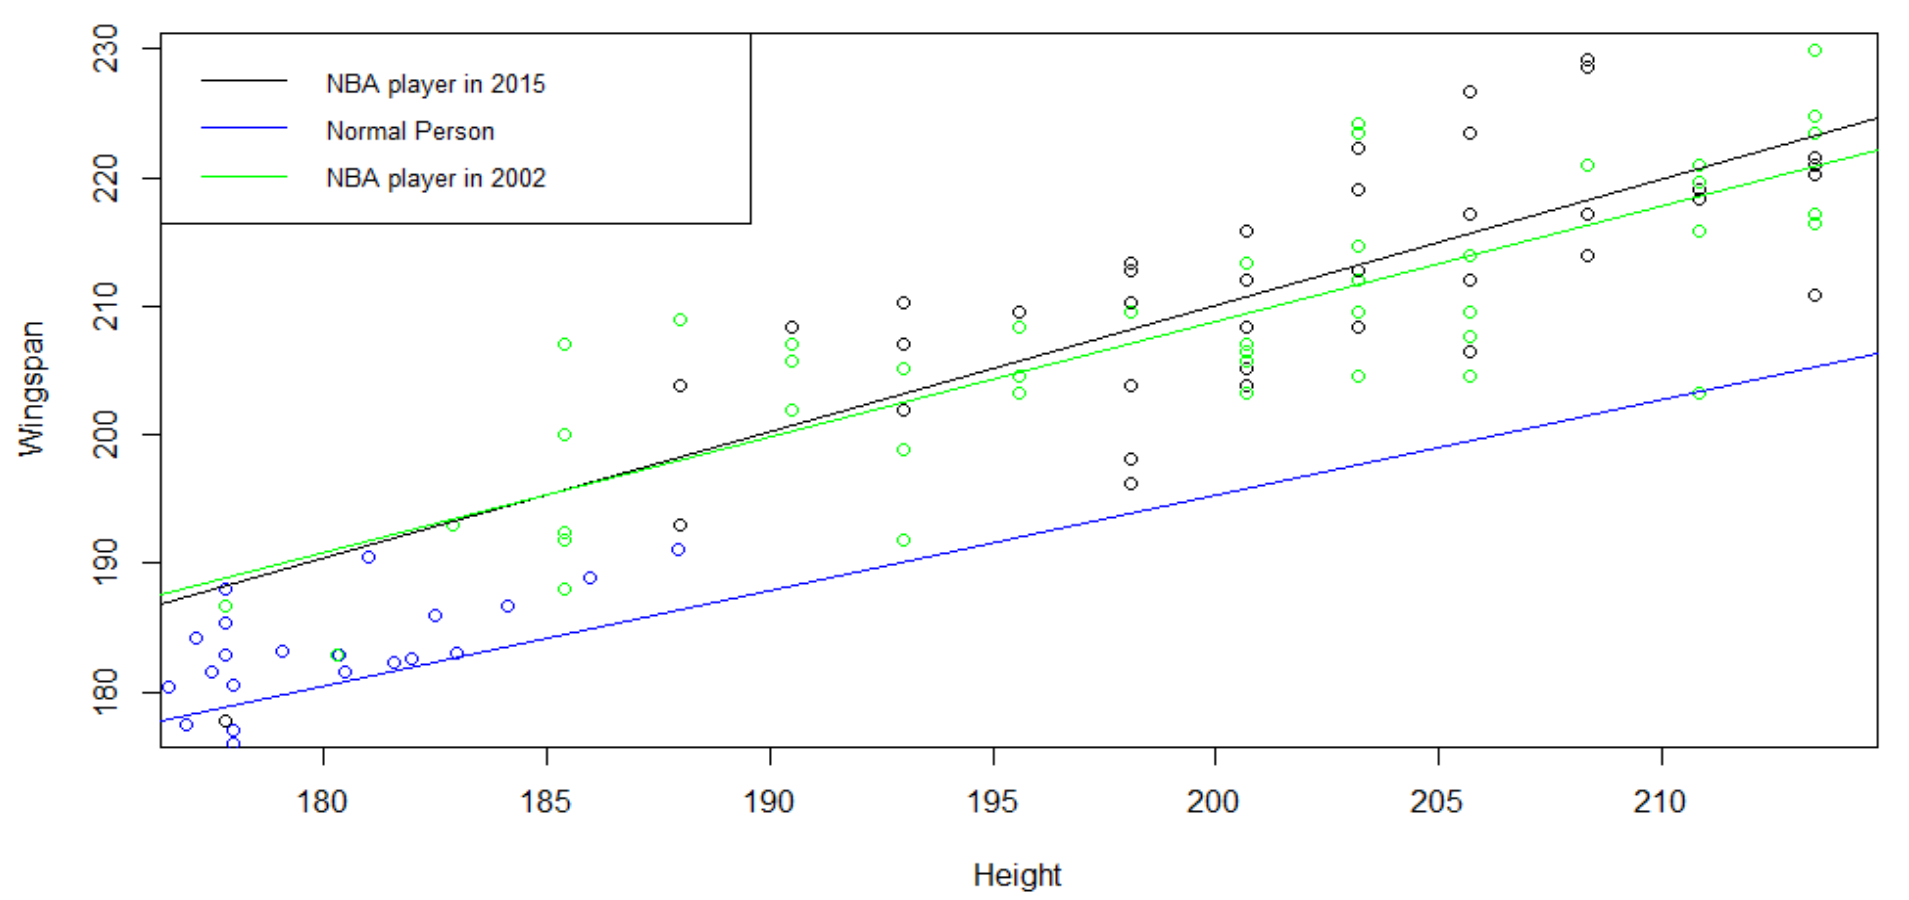
\includegraphics[trim = 0 0 0 0,clip,width=0.85\textwidth]{figures/heightvswingspan.png} }
    \end{center}
    \label{sec:Summary of Sample}
    \hrule
\end{figure}

\vspace{2.5mm}

\noindent Clearly, we can see from the plot that NBA Height and Wingspan
in both 2015 and 2002 are significantly larger than the normal males
height and weight. \vspace{2.5mm}

\noindent The lines of NBA players in 2015 and 2012 are very close and
it is difficult to make any assumptions.

\newpage

\subsection{Summary Statistics of Data}

\noindent Correlation Table is on Next Page \newpage
\begin{sidewaystable}[!htbp]
\footnotesize
\centering
\caption{\textbf{NBA Descriptive Statistics and Correlation Analysis}}
\label{table:correlation-NBA}
\begin{tabularx}{.9\textwidth}{{r@{ \ \ } p{35mm} r@{}lp{1mm} r@{}l p{5mm} r@{}l p{2mm} r@{}l p{2mm} r@{}l p{2mm} r@{}l p{2mm} r@{}l p{2mm} r@{}l p{2mm} r@{}l p{2mm} r@{}l p{2mm}   r@{}l  }}
 & \\
\hline
 & \\
\multicolumn{2}{c}{\textbf{ }} & \multicolumn{2}{c}{\textbf{M}} & & \multicolumn{2}{c}{\textbf{SD}} &  & \multicolumn{2}{c}{\textbf{1}} &  & \multicolumn{2}{c}{\textbf{2}} &  & \multicolumn{2}{c}{\textbf{3}} &  & \multicolumn{2}{c}{\textbf{4}} &  & \multicolumn{2}{c}{\textbf{5}} &  & \multicolumn{2}{c}{\textbf{6}} &  & \multicolumn{2}{c}{\textbf{7}} &  & \multicolumn{2}{c}{\textbf{8}} &  & \\ 
 & \\
\hline
 & \\
\textbf{1} & \textbf{height.NA} &  174&.4 &  &  7&.75 &  &  1&  &  &  \multicolumn{2}{c}{ \  \  \  \  \ }  &  &  \multicolumn{2}{c}{ \  \  \  \  \ }  &  &  \multicolumn{2}{c}{ \  \  \  \  \ }  &  &  \multicolumn{2}{c}{ \  \  \  \  \ }  &  &  \multicolumn{2}{c}{ \  \  \  \  \ }  &  &  \multicolumn{2}{c}{ \  \  \  \  \ }  &  &  \multicolumn{2}{c}{ \  \  \  \  \ }  &  & \\ 
 & \\
\textbf{2} & \textbf{arm.span.NA} &  176&.3 &  &  8&.59 &  &  &.67{$^{***}$}  &  &  1&  &  &  \multicolumn{2}{c}{ \  \  \  \  \ }  &  &  \multicolumn{2}{c}{ \  \  \  \  \ }  &  &  \multicolumn{2}{c}{ \  \  \  \  \ }  &  &  \multicolumn{2}{c}{ \  \  \  \  \ }  &  &  \multicolumn{2}{c}{ \  \  \  \  \ }  &  &  \multicolumn{2}{c}{ \  \  \  \  \ }  &  & \\ 
 & \\
\textbf{3} & \textbf{Measure Ape Scale} &  1&.0 &  &  &.04 &  &  -&.32{$^{*}$}  &  &  &.49{$^{***}$}  &  &  1&  &  &  \multicolumn{2}{c}{ \  \  \  \  \ }  &  &  \multicolumn{2}{c}{ \  \  \  \  \ }  &  &  \multicolumn{2}{c}{ \  \  \  \  \ }  &  &  \multicolumn{2}{c}{ \  \  \  \  \ }  &  &  \multicolumn{2}{c}{ \  \  \  \  \ }  &  & \\ 
 & \\
\textbf{4} & \textbf{Height (in cm) 2002} &  201&.1 &  &  9&.89 &  &  -&.17 &  &  -&.13 &  &  &.05 &  &  1&  &  &  \multicolumn{2}{c}{ \  \  \  \  \ }  &  &  \multicolumn{2}{c}{ \  \  \  \  \ }  &  &  \multicolumn{2}{c}{ \  \  \  \  \ }  &  &  \multicolumn{2}{c}{ \  \  \  \  \ }  &  & \\ 
 & \\
\textbf{5} & \textbf{Wingspan (in cm) 2002} &  211&.0 &  &  10&.08 &  &  -&.10 &  &  -&.07 &  &  &.03 &  &  &.86{$^{***}$}  &  &  1&  &  &  \multicolumn{2}{c}{ \  \  \  \  \ }  &  &  \multicolumn{2}{c}{ \  \  \  \  \ }  &  &  \multicolumn{2}{c}{ \  \  \  \  \ }  &  & \\ 
 & \\
\textbf{6} & \textbf{NBA Ape Scale 2002} &  1&.0 &  &  &.03 &  &  &.14 &  &  &.11 &  &  -&.03 &  &  -&.31{$^{*}$}  &  &  &.21 &  &  1&  &  &  \multicolumn{2}{c}{ \  \  \  \  \ }  &  &  \multicolumn{2}{c}{ \  \  \  \  \ }  &  & \\ 
 & \\
\textbf{7} & \textbf{Height (in cm) 2015} &  202&.0 &  &  7&.55 &  &  -&.11 &  &  -&.35{$^{*}$}  &  &  -&.31{$^{*}$}  &  &  -&.12 &  &  -&.17 &  &  -&.09 &  &  1&  &  &  \multicolumn{2}{c}{ \  \  \  \  \ }  &  & \\ 
 & \\
\textbf{8} & \textbf{Wingspan (in cm) 2015} &  212&.0 &  &  9&.60 &  &  -&.03 &  &  -&.26{$^{\dagger}$}  &  &  -&.31{$^{*}$}  &  &  &.08 &  &  -&.04 &  &  -&.25{$^{\dagger}$}  &  &  &.77{$^{***}$}  &  &  1&  &  & \\ 
 & \\
\textbf{9} & \textbf{NBA Ape Scale 2015} &  1&.0 &  &  &.03 &  &  &.11 &  &  &.04 &  &  -&.09 &  &  &.28{$^{*}$}  &  &  &.15 &  &  -&.27{$^{\dagger}$}  &  &  -&.07 &  &  &.58{$^{***}$}  &  & \\ 
 & \\
\hline
 & \\
\multicolumn{31}{p{0.9\textwidth}}{  \footnotesize { \begin{hangparas}{0.75in}{1} \textbf{\underline{Notes}:} \ \ Pearson pairwise correlations are reported; \newline a two-side test was performed to report correlation significance.  \end{hangparas} } }  & \\  
\multicolumn{31}{p{0.9\textwidth}}{  {\tiny {$^{\dagger} p < .10$} }  {     } {\tiny        {$^{*} p < .05$} }  {     } {\tiny       {$^{**} p < .01$} }  {     } {\tiny      {$^{***} p < .001$} } {     }     } & \\ 
 & \\
\hline
\end{tabularx}
\end{sidewaystable}


\label{sec:data-summary}

\newpage

\section{Key Findings}
\label{sec:findings}

From my correlation table I have several correlating pairs.

\noindent For Normal Males: \noindent Wingspan correlates with height
corr=.67

\noindent For NBA players in 2015: Wingspan correlates with height
corr=.86

\noindent For NBA players in 2002: Wingspan correlates with height
corr=.77

\vspace{5mm}

\noindent Is there a strong relationship between height and arm span?
\newline

\noindent These three correlations tell me that Wingspan and Height have
a strong positive relationship.

\noindent Additionally, if we take a look at the mean of wingspan in any
of the datasets, It is not very different than the height. \newline
\noindent I can conclude that the relationship Wingspan and Height is
strong.

\vspace{5mm}

\noindent Has the ratio between height and arm span changed over time
for NBA Players? \newline

\noindent I found the ape index of both NBA datasets (2002, 2015):
\newline \noindent NBA ape index 2002: 1.0449 \newline \noindent NBA ape
index 2015: 1.0495 \newline \noindent There is no significant difference
between Ape index of NBA players who played before or during the 2002
season and from NBA players who played after the 2015 season.

\vspace{5mm}

\noindent How does the ratio between height and arm span compare between
NBA players and normal males? \newline

\noindent Since ape index is extremely close in the NBA data I can just
average it out as one NBA ape index to compare to the normal males ape
index. \newline \noindent I found the average ape index of both NBA
datasets (2002, 2015): \newline \noindent Average NBA ape index
(2002,2015): 1.0472 \newline \noindent Male ape index: 1.0112 \newline
\noindent The ape index of NBA players is slightly higher than the
normals males.

\newpage
\section{Conclusion}
\label{sec:conclusion}

\noindent I set out to answer 3 questions: \newline \noindent Is there a
strong relationship between height and arm span? \newline \noindent Has
the ratio between height and arm span changed over time for NBA Players?
\newline \noindent How does the ratio between height and arm span
compare between NBA players and normal males? \newline \newline
\indent From my research and analysis I can conclude that there is in
fact a strong relationship between height and arm span. They seem to be
highly correlated. It seems as height increases, arm span increases and
I am not very surprised with these results because typically the human
body's wingspan is the same as their height. This theory is taken from
Leonardo da Vinci. \vspace{5mm}

To answer my next two questions I found the proportion between ape scale
and height which is known as ``ape index''. I compared this ape index
score between my two NBA measurement samples and they turned out to be
almost identical in ape index. From this I can conclude: there is no
significant change over time between NBA player proportions of height to
wingspan. \vspace{5mm}

Finally, I wanted to know how the proportion of height and wingspan
differed between normal males and NBA players. From my samples of 49
observations, I was not able to find a significant difference. Although
ape index was larger for NBA players than normal males, I cannot safely
conclude that NBA players have larger indexes.

\newpage
\section{APPENDICES}
\label{sec:appendix}

\subsection{Data Provenance}
\label{sec:appendix-data-provenance}

My measurement data which came from those that have filled out the
handout consists of 428 rows and 37 columns. This data contains both
numerical and categorical data. I filtered the data to only include Male
samples of at least 18 years old. It is my belief this is an appropriate
age to select since the current minimum age to play in the NBA is 18.
After data cleansing, data wrangling and filtering, I was left with 49
observations to work with. I went from 126 rows to 49 after removing all
outliers, which points to the much of the data being inaccurate.
\newline \newline

My NBA dataset that came from Kaggle is titled ``NBA Players -
Measurements (1947-2017).'' The data set included 4551 rows and 18
columns. I was able to find a popular dataset that was publicly shared
by Fernando Blanco on Kaggle. The Data represents numerous body
measurements of players who have were in the NBA from 1947, all the way
to 2017. I split my data into two seperate data sets: NBA players who
played before or during the 2002 season and NBA players who played after
the 2015 season. From these two data pools, I took random samples of 49
observations to match the number of observations from my measurement
data. I also made a final merged dataset, In which I merged my 3
datasets and used in my analysis. \newline \newline

\subsection{Correlation Table}
\label{sec:Summary Statistics of Data}

The correlation table was made by running the function
BuildLatexCorrelationTable(). This function was made by instructor:
Monte Shaffer. The code to run the correlation table is in another file,
however the output of the function which is a .tex file is already
stored in a tables folder. \newline \newline

\subsection{Kaggle Reference}
\label{sec:References}

Kaggle is a data science community website that offers thousands of
\#datasets. \newline
\url{https://www.kaggle.com/whitefero/nba-players-measurements-19472017}
\newline \vspace{2.5mm} Vitruvian Drawing by Leonardo da Vinci \newline
\url{https://en.wikipedia.org/wiki/Vitruvian_Man}

\newpage
\subsubsection{Data Collection Handout}
\label{sec:appendix-data-handout}

\begin{figure}[!ht]
    \hrule
    \caption{ \textbf{Handout Page 1} }
    \begin{center}
        \scalebox{1.00}{    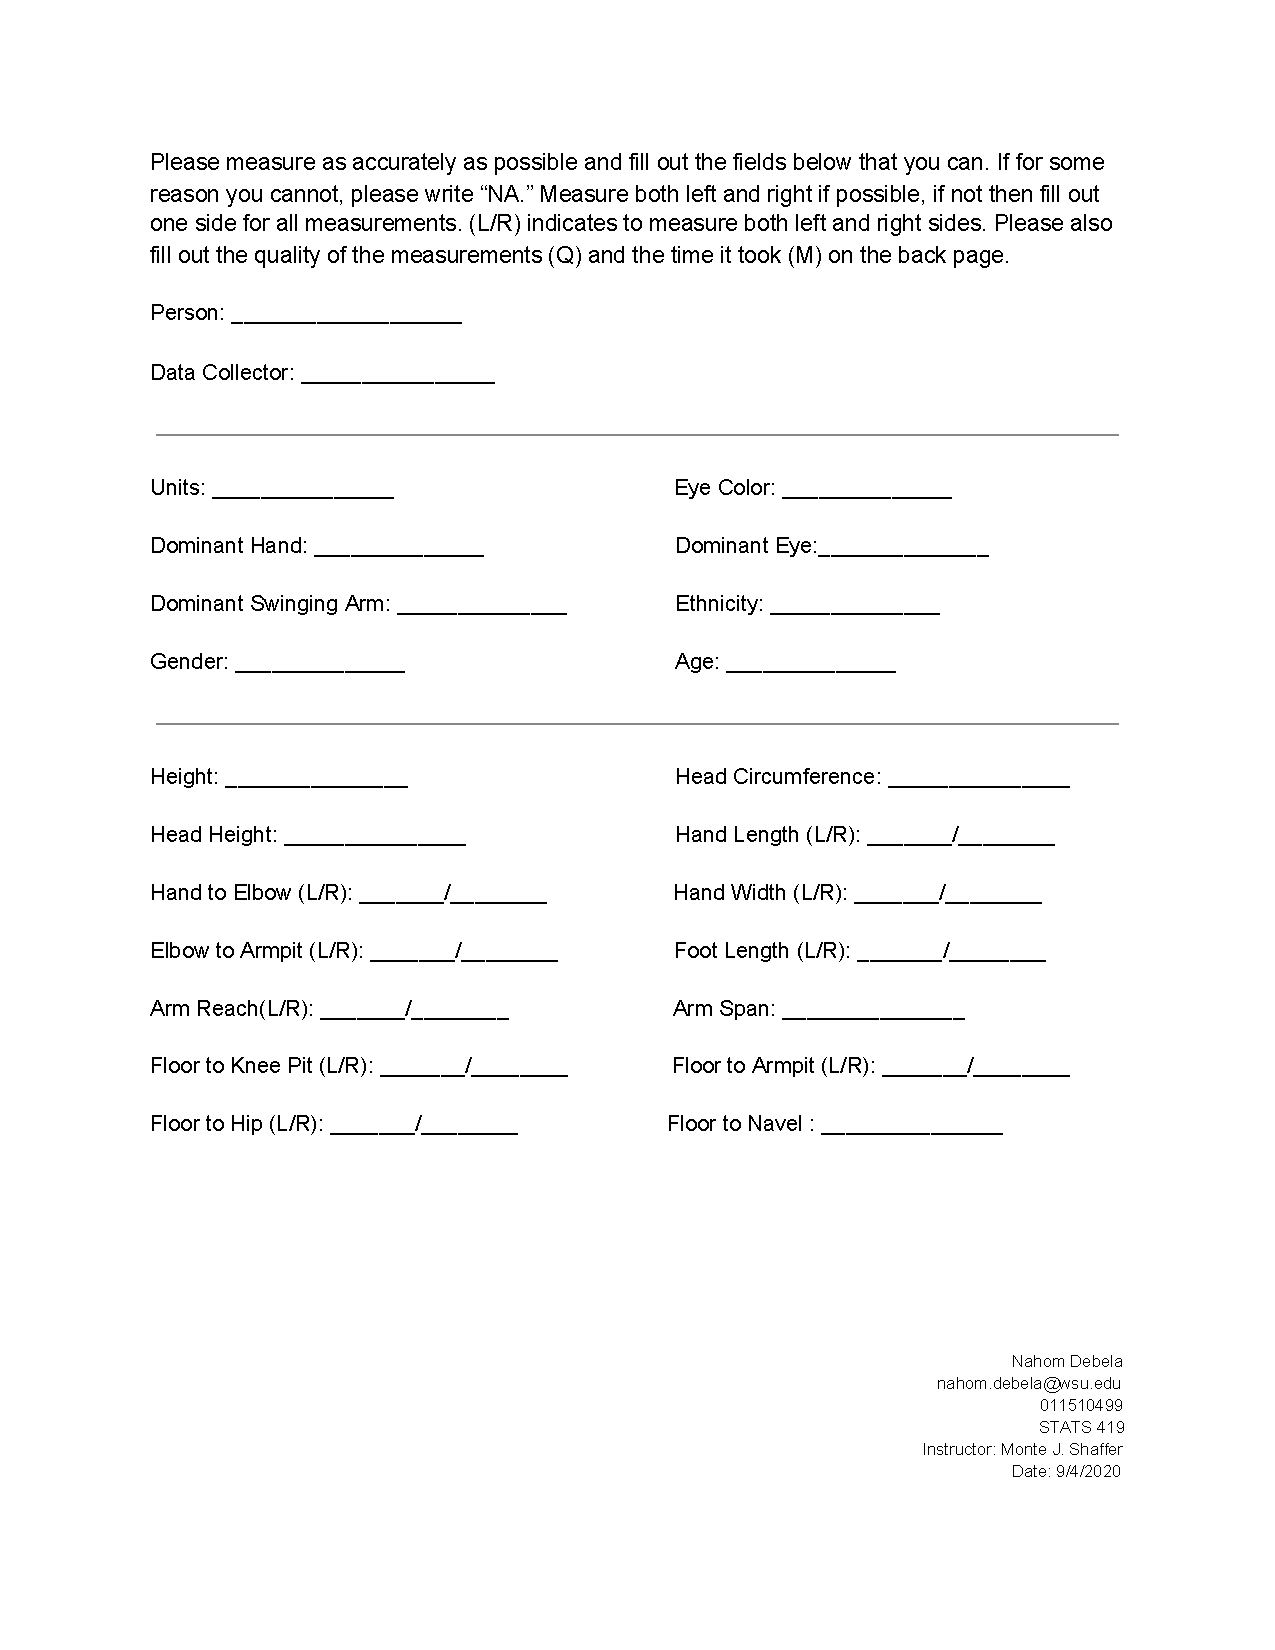
\includegraphics[trim = 0 0 0 0,clip,width=0.85\textwidth]{pdfs/handout1.pdf} }
    \end{center}
    \label{fig:handout-1}
    \hrule
\end{figure}

\newpage

\begin{figure}[!ht]
    \hrule
    \caption{ \textbf{Handout Page 2} }
    \begin{center}
        \scalebox{1.00}{    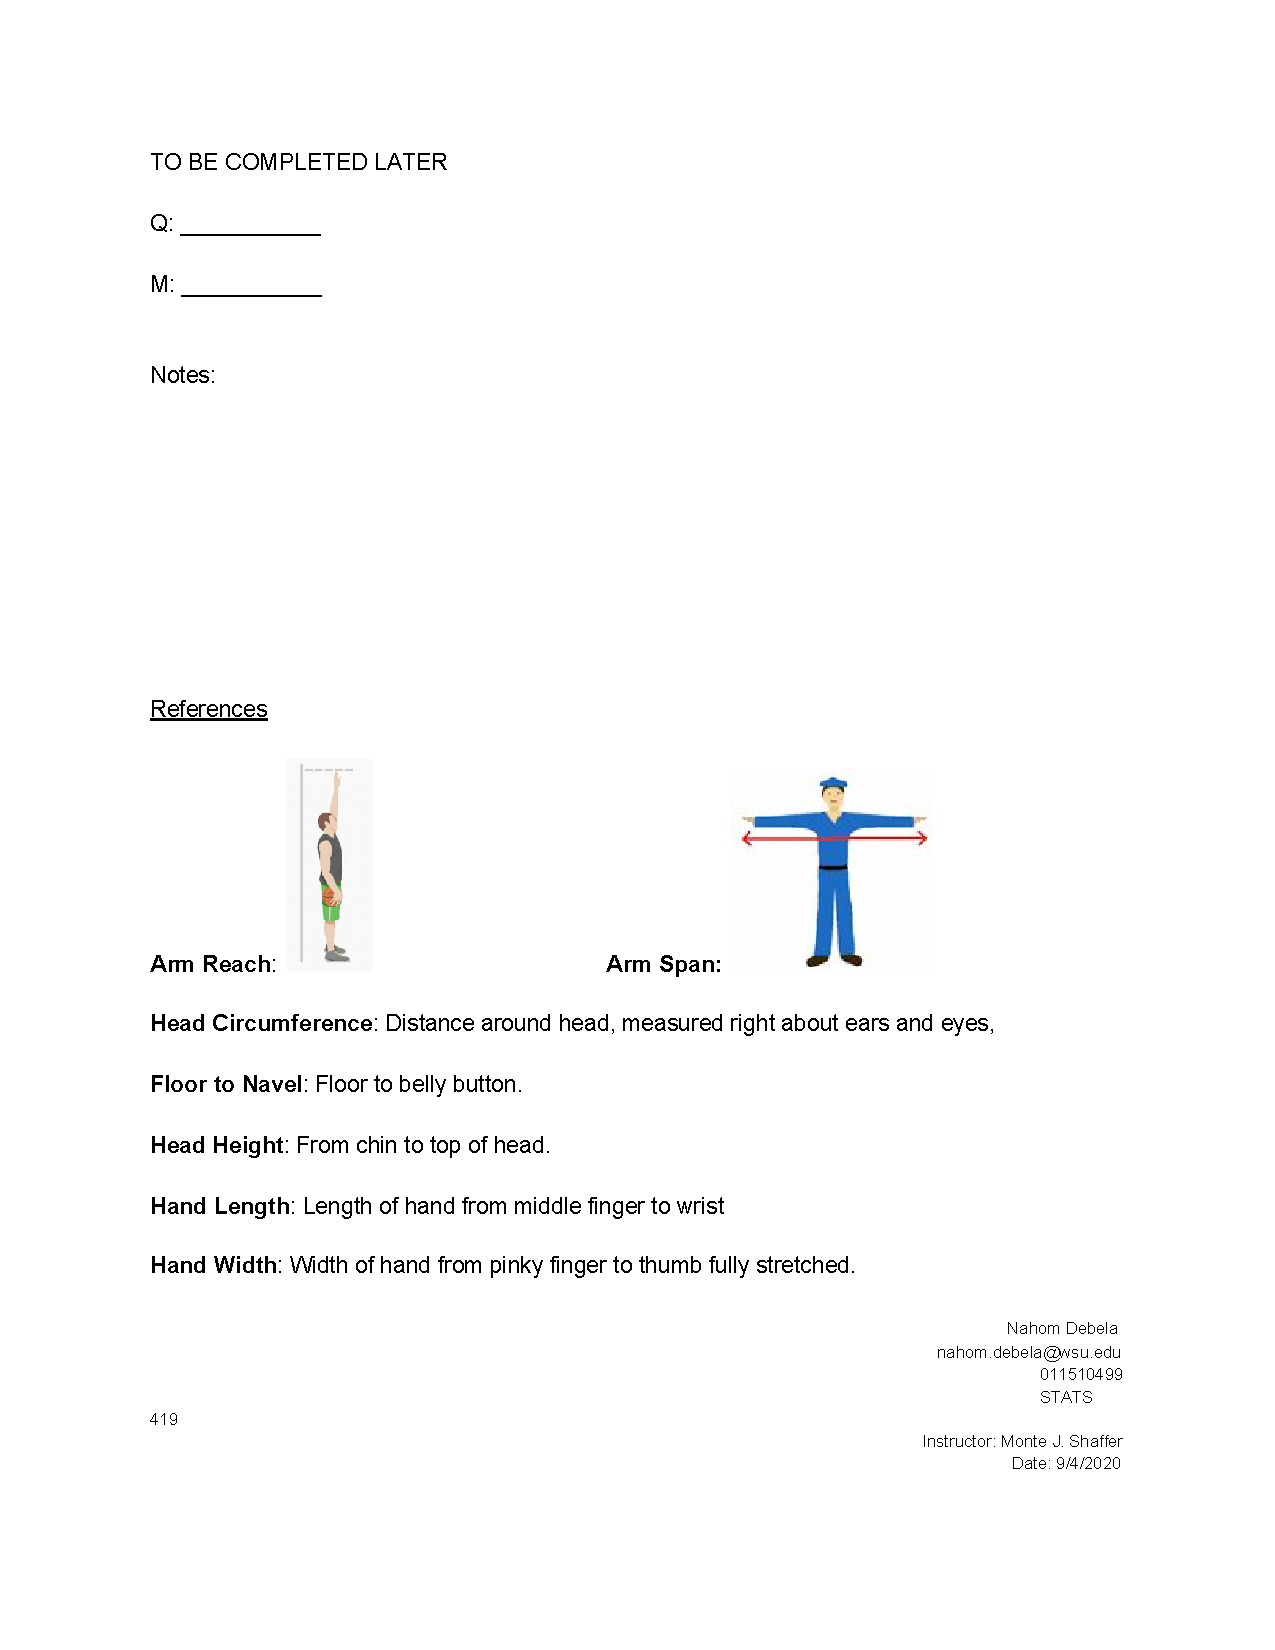
\includegraphics[trim = 0 0 0 0,clip,width=0.85\textwidth]{pdfs/handout2.pdf} }
    \end{center}
    \label{fig:handout-2}
    \hrule
\end{figure}

\newpage

\subsection{Preparing the Report Workspace as a subsection}
\label{sec:appendix-setup}

\subsubsection{Preparing the Report Workspace as a subsubsection}
\label{sec:appendix-setup2}

\paragraph{Preparing the Report Workspace as a paragraph}
\label{sec:appendix-setup3}

\subparagraph{Preparing the Report Workspace as a subparagrah}
\label{sec:appendix-setup4}

Below is the necessary functions and libraries required to run the code
referenced in this document.

\begin{Shaded}
\begin{Highlighting}[]
\KeywordTok{library}\NormalTok{(devtools) }\CommentTok{\# required for source\_url}
\NormalTok{my.source =}\StringTok{ \textquotesingle{}local\textquotesingle{}}\NormalTok{;}
\NormalTok{local.path =}\StringTok{ "C:/Users/nahom/\_git\_/WSU\_STATS419\_FALL2020/"}\NormalTok{;}
\NormalTok{local.data.path.to.secret =}\StringTok{ "C:/Users/nahom/Desktop/STATS 419/datasets/measure/"}\NormalTok{;}
\NormalTok{local.data.path.to.secret.NBA =}\StringTok{ "C:/Users/nahom/Desktop/STATS 419/datasets/measure{-}NBA/"}
\KeywordTok{source}\NormalTok{( }\KeywordTok{paste0}\NormalTok{(local.path, }\StringTok{"functions/libraries.R"}\NormalTok{), }\DataTypeTok{local =}\NormalTok{ T);}

\KeywordTok{library}\NormalTok{(humanVerseWSU);}
\NormalTok{path.github =}\StringTok{ "https://raw.githubusercontent.com/MonteShaffer/humanVerseWSU/master/"}\NormalTok{;}
\KeywordTok{source\_url}\NormalTok{(}\StringTok{"https://raw.githubusercontent.com/MonteShaffer/humanVerseWSU/master/humanVerseWSU/R/functions{-}dataframe.R"}\NormalTok{);}
\CommentTok{\# EDA functions}
\KeywordTok{source\_url}\NormalTok{( }\KeywordTok{paste0}\NormalTok{(path.github,}\StringTok{"humanVerseWSU/R/functions{-}EDA.R"}\NormalTok{) );  }\CommentTok{\#  }
\KeywordTok{source}\NormalTok{( }\KeywordTok{paste0}\NormalTok{(local.path, }\StringTok{"functions/functions{-}project{-}measure.R"}\NormalTok{), }\DataTypeTok{local =}\NormalTok{ T);}
\end{Highlighting}
\end{Shaded}

Below is the code to load the data and prepare it for analysis.

\begin{Shaded}
\begin{Highlighting}[]
\NormalTok{measure.uncleaned =}\StringTok{ }\KeywordTok{readData}\NormalTok{(}\StringTok{"measure{-}students.txt"}\NormalTok{)}
\NormalTok{measure.cleaned =}\StringTok{ }\KeywordTok{dataCleaning}\NormalTok{(measure.uncleaned)}

\NormalTok{nbaData.uncleaned =}\StringTok{ }\KeywordTok{readDataNBA}\NormalTok{(}\StringTok{"Player {-} Bio Stats (1947{-}2017).csv"}\NormalTok{)}
\NormalTok{nbaData.cleaned}\FloatTok{.2015}\NormalTok{ =}\StringTok{ }\KeywordTok{cleanNbaData2015}\NormalTok{(nbaData.uncleaned)}
\NormalTok{nbaData.cleaned}\FloatTok{.2002}\NormalTok{ =}\StringTok{ }\KeywordTok{cleanNbaData2002}\NormalTok{(nbaData.uncleaned)}
\end{Highlighting}
\end{Shaded}

Below is the code I used in my analysis and plots

\begin{Shaded}
\begin{Highlighting}[]
\CommentTok{\# For summary tables}
\CommentTok{\# I called get\_summary() function}
\CommentTok{\# get\_summary(measure.cleaned.df,nbaData.2002,nbaData.2015)}

\CommentTok{\# For height vs wingspan plot}
\CommentTok{\# I called displayPlotHeightWing}
\CommentTok{\# displayPlotHeightWing(measure.cleaned.df,nbaData.2015,nbaData.2002)}
\end{Highlighting}
\end{Shaded}





%% appendices go here!


\newpage
\theendnotes

%%%%%%%%%%%%%%%%%%%%%%%%%%%%%%%%%%%  biblio %%%%%%%%
\newpage
\begin{auxmulticols}{2}
\singlespacing 
\bibliography{./../biblio/master.bib}

%%%%%%%%%%%%%%%%%%%%%%%%%%%%%%%%%%%  biblio %%%%%%%%
\end{auxmulticols}

\newpage
{
\hypersetup{linkcolor=black}
\setcounter{tocdepth}{3}
\tableofcontents
}



\end{document}